% questions.tex —— 2007 年·上海卷·理科 · 题目内容片段（无答案）
% 由 tools/generate_projects.py 依来源总账自 2007/2007_数学真题_上海理_试题.md 生成，勿手改（改源 MD 后重跑）


状态：needs-review；依固定 PDF 两页图像转录，图形已矢量重绘，正式构建与逐页验收待完成。源未列各题分值，不补分值。

\gkpart{一、填空题}

\begin{question}
\gkti{1}函数 $f(x)=\frac{\lg(4-x)}{x-3}$ 的定义域是\gkblank{}。
\end{question}
\begin{question}
\gkti{2}若直线 $l_1:2x+my+1=0$ 与直线 $l_2:y=3x-1$ 平行，则 $m=$\gkblank{}。
\end{question}
\begin{question}
\gkti{3}函数 $f(x)=\frac{x}{x-1}$ 的反函数 $f^{-1}(x)=$\gkblank{}。
\end{question}
\begin{question}
\gkti{4}方程 $9^x-6\cdot3^x-7=0$ 的解是\gkblank{}。
\end{question}
\begin{question}
\gkti{5}若 $x,y\in\mathbb R^+$，且 $x+4y=1$，则 $x\cdot y$ 的最大值是\gkblank{}。
\end{question}
\begin{question}
\gkti{6}函数 $y=\sin(x+\frac\pi3)\sin(x+\frac\pi2)$ 的最小正周期 $T=$\gkblank{}。
\end{question}
\begin{question}
\gkti{7}在五个数字 1，2，3，4，5 中，若随机取出三个数字，则剩下两个数字都是奇数的概率是\gkblank{}。（结果用数值表示）
\end{question}
\begin{question}
\gkti{8}以双曲线 $\frac{x^2}{4}-\frac{y^2}{5}=1$ 的中心为焦点，且以该双曲线的左焦点为顶点的抛物线方程是\gkblank{}。
\end{question}
\begin{question}
\gkti{9}对于非零实数 $a,b$，以下四个命题都成立：① $a+\frac1a\ne0$；② $(a+b)^2=a^2+2ab+b^2$；③ 若 $|a|=|b|$，则 $a=\pm b$；④ 若 $a^2=ab$，则 $a=b$。那么，对于非零复数 $a,b$，仍然成立的命题的所有序号是\gkblank{}。
\end{question}
\begin{question}
\gkti{10}在平面上，两条直线的位置关系有相交、平行、重合三种。已知 $\alpha,\beta$ 是两个相交平面，空间两条直线 $l_1,l_2$ 在 $\alpha$ 上的射影是直线 $s_1,s_2$，$l_1,l_2$ 在 $\beta$ 上的射影是直线 $t_1,t_2$。用 $s_1$ 与 $s_2$、$t_1$ 与 $t_2$ 的位置关系，写出一个总能确定 $l_1$ 与 $l_2$ 是异面直线的充分条件：\gkblank{}。
\Needspace{0.4\textheight}
\end{question}
\begin{question}
\gkti{11}已知 $P$ 为圆 $x^2+(y-1)^2=1$ 上任意一点（原点 $O$ 除外），直线 $OP$ 的倾斜角为 $\theta$ 弧度，记 $d=|OP|$。在右侧的坐标系中，画出以 $(\theta,d)$ 为坐标的点的轨迹的大致图形为 
\nopagebreak[4]
\begin{center}% Candidate; source page 405; blank answering grid, not solution curve.
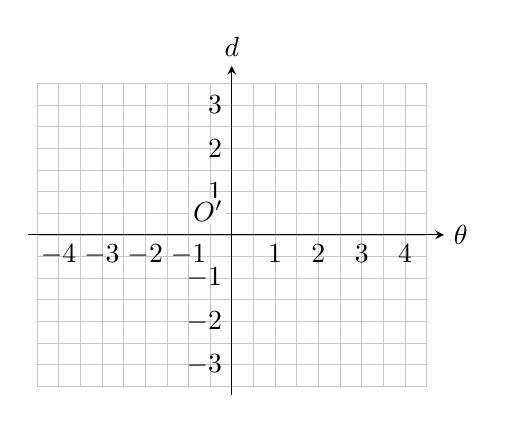
\begin{tikzpicture}[x=.55cm,y=.55cm,>=stealth]
\draw[step=.5,gray!45,very thin] (-4.5,-3.5) grid (4.5,3.5);
\draw[->] (-4.7,0)--(4.9,0) node[right] {$\theta$};
\draw[->] (0,-3.7)--(0,3.9) node[above] {$d$};
\foreach \x in {-4,-3,-2,-1,1,2,3,4} \node[below] at (\x,0) {$\x$};
\foreach \y in {-3,-2,-1,1,2,3} \node[left] at (0,\y) {$\y$};
\node[fill=white,inner sep=1pt] at (-.55,.55) {$O'$};
\end{tikzpicture}
\end{center}
\nopagebreak[4]
\end{question}
\gkpart{二、选择题}

\begin{question}
\gkti{12}已知 $a,b\in\mathbb R$，且 $2+ai,b+i$（$i$ 是虚数单位）是实系数一元二次方程 $x^2+px+q=0$ 的两个根，那么 $p,q$ 的值分别是（ ）。

（A）$p=-4,q=5$；

（B）$p=-4,q=3$；

（C）$p=4,q=5$；

（D）$p=4,q=3$。
\end{question}
\begin{question}
\gkti{13}设 $a,b$ 是非零实数，若 $a<b$，则下列不等式成立的是（ ）。

（A）$a^2<b^2$；

（B）$ab^2<a^2b$；

（C）$\frac1{ab^2}<\frac1{a^2b}$；

（D）$\frac ba<\frac ab$。
\end{question}
\begin{question}
\gkti{14}直角坐标系 $xOy$ 中，$\vec i,\vec j$ 分别是与 $x,y$ 轴正方向同向的单位向量。在直角三角形 $ABC$ 中，若 $\overrightarrow{AB}=2\vec i+\vec j$，$\overrightarrow{AC}=3\vec i+k\vec j$，则 $k$ 的可能值个数是（ ）。

（A）1；

（B）2；

（C）3；

（D）4。
\end{question}
\begin{question}
\gkti{15}设 $f(x)$ 是定义在正整数集上的函数，且 $f(x)$ 满足：“当 $f(k)\ge k^2$ 成立时，总可推出 $f(k+1)\ge(k+1)^2$ 成立”。那么，下列命题成立的是（ ）。

（A）若 $f(3)\ge9$ 成立，则当 $k\ge1$ 时，均有 $f(k)\ge k^2$ 成立。

（B）若 $f(5)\ge25$ 成立，则当 $k\le5$ 时，均有 $f(k)\ge k^2$ 成立。

（C）若 $f(7)<49$ 成立，则当 $k\ge8$ 时，均有 $f(k)<k^2$ 成立。

（D）若 $f(4)=25$ 成立，则当 $k\ge4$ 时，均有 $f(k)\ge k^2$ 成立。

\end{question}
\gkpart{三、解答题}

\Needspace{0.4\textheight}
\begin{question}
\gkti{16}如图，在体积为 1 的直三棱柱 $ABC-A_1B_1C_1$ 中，$\angle ACB=90^\circ$，$AC=BC=1$，求直线 $A_1B$ 与平面 $BB_1C_1C$ 所成角。（结果用反三角函数值表示）
\nopagebreak[4]
\begin{center}% Candidate; source page 405. Dashed edges meet at hidden C.
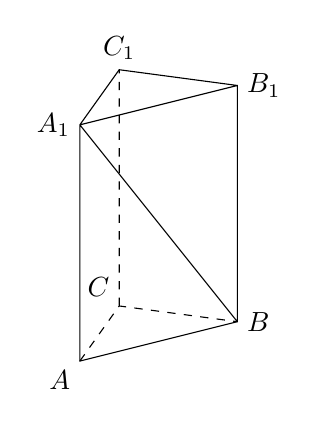
\begin{tikzpicture}[scale=1,>=stealth]
\coordinate (A) at (0,0); \coordinate (B) at (2,.5); \coordinate (C) at (.5,.7);
\coordinate (A1) at (0,3); \coordinate (B1) at (2,3.5); \coordinate (C1) at (.5,3.7);
\draw (A)--(B)--(B1)--(A1)--cycle (A1)--(C1)--(B1) (A1)--(B);
\draw[dashed] (A)--(C)--(B) (C)--(C1);
\node[below left] at (A) {$A$}; \node[right] at (B) {$B$}; \node[above left] at (C) {$C$};
\node[left] at (A1) {$A_1$}; \node[right] at (B1) {$B_1$}; \node[above] at (C1) {$C_1$};
\end{tikzpicture}
\end{center}
\nopagebreak[4]
\end{question}
\begin{question}
\gkti{17}在 $\triangle ABC$ 中，$a,b,c$ 分别是三个内角 $A,B,C$ 的对边。若 $a=2,C=\frac\pi4,\cos\frac B2=\frac{2\sqrt5}{5}$，求 $\triangle ABC$ 的面积 $S$。
\end{question}
\begin{question}
\gkti{18}近年来，太阳能技术运用的步伐日益加快。2002 年全球太阳电池的年生产量达到 670 兆瓦，年生产量的增长率为 34\%。以后四年中，年生产量的增长率逐年递增 2\%（如，2003 年的年生产量的增长率为 36\%）。
（1）求 2006 年全球太阳电池的年生产量（结果精确到 0.1 兆瓦）；
（2）目前太阳电池产业存在的主要问题是市场安装量远小于生产量，2006 年的实际安装量为 1420 兆瓦。假设以后若干年内太阳电池的年生产量的增长率将保持在 42\%，到 2010 年，要使年安装量与年生产量基本持平（即年安装量不少于年生产量的 95\%），这四年中太阳电池的年安装量的平均增长率至少应达到多少（结果精确到 0.1\%）？
\end{question}
\begin{question}
\gkti{19}已知函数 $f(x)=x^2+\frac ax$（$x\ne0$，常数 $a\in\mathbb R$）。
（1）讨论函数 $f(x)$ 的奇偶性，并说明理由；
（2）若函数 $f(x)$ 在 $x\in[2,+\infty)$ 上为增函数，求 $a$ 的取值范围。
\end{question}
\begin{question}
\gkti{20}如果有穷数列 $a_1,a_2,a_3,\ldots,a_n$（$n$ 为正整数）满足条件 $a_1=a_n,a_2=a_{n-1},\ldots,a_n=a_1$，即 $a_i=a_{n-i+1}$（$i=1,2,\ldots,n$），我们称其为“对称数列”。例如，由组合数组成的数列 $C_m^0,C_m^1,\ldots,C_m^m$ 就是“对称数列”。
（1）设 $\{b_n\}$ 是项数为 7 的“对称数列”，其中 $b_1,b_2,b_3,b_4$ 是等差数列，且 $b_1=2,b_4=11$。依次写出 $\{b_n\}$ 的每一项；
（2）设 $\{c_n\}$ 是项数为 $2k-1$（正整数 $k>1$）的“对称数列”，其中 $c_k,c_{k+1},\ldots,c_{2k-1}$ 是首项为 50、公差为 $-4$ 的等差数列。记 $\{c_n\}$ 各项的和为 $S_{2k-1}$。当 $k$ 为何值时，$S_{2k-1}$ 取得最大值？并求出 $S_{2k-1}$ 的最大值；
（3）对于确定的正整数 $m>1$，写出所有项数不超过 $2m$ 的“对称数列”，使得 $1,2,2^2,\ldots,2^{m-1}$ 依次是该数列中连续的项；当 $m>1500$ 时，求其中一个“对称数列”前 2008 项的和 $S_{2008}$。
\Needspace{0.4\textheight}
\end{question}
\begin{question}
\gkti{21}我们把由半椭圆 $\frac{x^2}{a^2}+\frac{y^2}{b^2}=1$（$x\ge0$）与半椭圆 $\frac{y^2}{b^2}+\frac{x^2}{c^2}=1$（$x\le0$）合成的曲线称作“果圆”，其中 $a^2=b^2+c^2,a>0,b>c>0$。如图，设点 $F_0,F_1,F_2$ 是相应椭圆的焦点，$A_1,A_2$ 和 $B_1,B_2$ 分别是“果圆”与 $x,y$ 轴的交点。
（1）若 $\triangle F_0F_1F_2$ 是边长为 1 的等边三角形，求“果圆”的方程；
（2）当 $|A_1A_2|>|B_1B_2|$ 时，求 $\frac bc$ 的取值范围；
（3）连接“果圆”上任意两点的线段称为“果圆”的弦。试研究：是否存在实数 $k$，使斜率为 $k$ 的“果圆”平行弦的中点轨迹总是落在某个椭圆上？若存在，求出所有可能的 $k$ 值；若不存在，说明理由。
\nopagebreak[4]
\begin{center}% Candidate schematic; a^2=b^2+c^2, b>c>0. Coordinates use c=1,b=1.3.
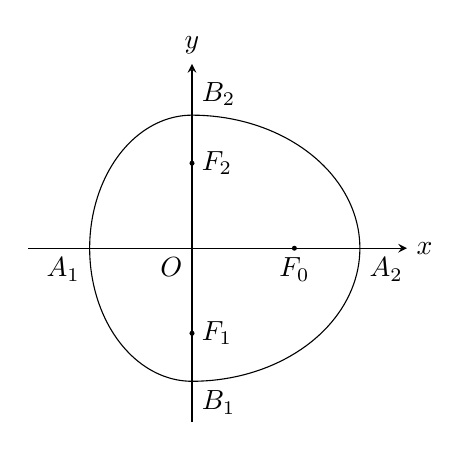
\begin{tikzpicture}[scale=1.3,>=stealth]
\draw[->] (-1.6,0)--(2.1,0) node[right] {$x$};
\draw[->] (0,-1.7)--(0,1.8) node[above] {$y$};
\draw plot[domain=-90:90,samples=81] ({sqrt(2.69)*cos(\x)},{1.3*sin(\x)});
\draw plot[domain=90:270,samples=81] ({cos(\x)},{1.3*sin(\x)});
\fill (1,0) circle (.7pt) node[below] {$F_0$};
\fill (0,{sqrt(.69)}) circle (.7pt) node[right] {$F_2$};
\fill (0,{-sqrt(.69)}) circle (.7pt) node[right] {$F_1$};
\node[below left] at (0,0) {$O$};
\node[below left] at (-1,0) {$A_1$}; \node[below right] at ({sqrt(2.69)},0) {$A_2$};
\node[below right] at (0,-1.3) {$B_1$}; \node[above right] at (0,1.3) {$B_2$};
\end{tikzpicture}
\end{center}
\nopagebreak[4]

\end{question}